\chapter{Experimental Framework}

\MyQuote{What we observe is not nature itself, but nature exposed to our method of
questioning.}{Werner Heisenberg}

In the previous Chapter, I have introduced the key features of the QCD, today's
theory of the strong interaction. A predictions of the QCD are tested at particle
accelerators persistently, with no signs for a new physics so far. 
Large Hadron Collider, which will open energy regions not observed yet, can
change this very soon.

The most prevailing objects, we observe at inelastic collisions on hadron
colliders, are collimated particle showers, called jets. With energies covering
a range from a few GeV to a few TeV, at the Large Hadron Collider, and with the
direct connection to the QCD processes, occurring during the collision, the jets
are a suitable candidates allowing testing the QCD up to its edges.

In this Chapter, I present the Large Hadron Collider and the ATLAS detector.
With the use of the QCD, defined in the previous Chapter, I give reasons for the
necessity of jets, and I define the jet algorithms allowing us to
straightforwardly recombine a
set of particles into jets. At the end of this Chapter, I describe the essential
steps, which has to be taken, to correctly reconstruct jets on the ATLAS
detector.

\section{The Large Hadron Collider and The ATLAS Detector}

CERN, the European Organization for Nuclear Research, is the largest particle
physics laboratory in the world, located near Geneva, at the border between
Switzerland and France. The current flagship project at CERN is a particle
accelerator called the Large Hadron Collider, which, together with the
ATLAS Detector, will be presented in this Section.

\subsection{The Large Hadron Collider}

The Large Hadron Collider (LHC) \cite{LHC, LHCPastPresentFuture} is a charged
particle accelerator, which was built in the areas formerly used by the Large
Electron-Positron Collider.  The main accelerator ring, of 27 km circumference,
is located around 100 m below the surface, with four main experiments located
around the ring: A Large Ion Collider Experiment (ALICE), A Toroidal LHC
ApparatuS (ATLAS), Compact Muon Solenoid (CMS) and Large Hadron Collider beauty
(LHCb). The complete accelerator and detector system is shown in
Figure~\ref{fig:LHC}.

\begin{figure}[t]
  \centering
  \includegraphics[width=\textwidth]{Chapter2/LHC.jpg}
  \caption[Diagram showing the locations of the four main experiments (ALICE,
          ATLAS, CMS and LHCb) that take place at the LHC. Located between 50 m and
          150 m underground, huge caverns have been excavated to house the giant
          detectors. The Super Proton Synchotron (SPS), the final link in the
          pre-acceleration chain, and its connection tunnels to the LHC, are also
          shown.]
          {Diagram showing the locations of the four main experiments (ALICE,
          ATLAS, CMS and LHCb) that take place at the LHC. Located between 50 m and
          150 m underground, huge caverns have been excavated to house the giant
          detectors. The Super Proton Synchotron (SPS), the final link in the
          pre-acceleration chain, and its connection tunnels to the LHC, are also
          shown.  Figure taken from~\cite{CERN:ATLASexperimentPictureswiki}.  }
  \label{fig:LHC}
\end{figure}

After 20 years of design, development, construction and testing, the LHC has
started to operate on November 23, 2009 and soon thereafter (March 30, 2010) the
proton-proton collisions achieved the center-of-mass energy $\sqrt{s} = 7 \TeV$,
which is a half of the design energy of the machine. On April 5, 2012, the
machine started its successful $\sqrt{s} = 8 \TeV$ run.

Next to the proton-proton collisions, first heavy-ion Pb-Pb collisions took place
in 2010 at a center-of-mass energy per pair of colliding nucleons $\sqrt{s} =
2.76 \TeV$. Proton-Pb collisions at $\sqrt{s} = 5.02 \TeV$, occurring on LHC
during 3 weeks of 2013, successfully demonstrated the LHC capability to provide
asymmetric collisions.  

The first running period of the LHC, Run~I, was very successful and resulted in
the discovery of the Higgs boson on July 4, 2012 \cite{HiggsDiscovery}.  The
accelerator complex, including its experiments, has been upgraded for two years
and the Run~II is expected to start in early summer 2015 \cite{LHCFuture,
LHCFutureLuminosigy}. In Run~II, the center-of-mass energy of proton-proton
collisions will be raised to $\sqrt{s} = 13 \TeV$, and the beam crossing time
is expected to be reduced from the current $50\,\text{ns}$ to $25\,\text{ns}$. The
integrated luminosity should be $\sim 100\,\text{fb}^{-1}$ after three years of
data collecting.

\subsection{The ATLAS Detector}

The ATLAS detector \cite{ATLAS} is a general-purpose detector surrounding one of
the interaction points of the LHC and, with $\sim 100$ million of individual
electronic channels, it is the most complicated instrument ever created.
The purpose of the ATLAS detector is to record particle collisions, up to the center-of-mass
energy per pair of colliding nucleons $\rts = 14 \TeV$. A detector overview is
shown in Figure~\ref{fig:ATLASfull}, where the main sub-detector systems can be
seen: the inner detector, used to reconstruct charged-particle tracks, the
electromagnetic calorimeters, the hadronic calorimeters, and the muon
spectrometer. 

\begin{figure}[p]
  \centering
  \begin{subfigure}[b]{0.9\textwidth}
    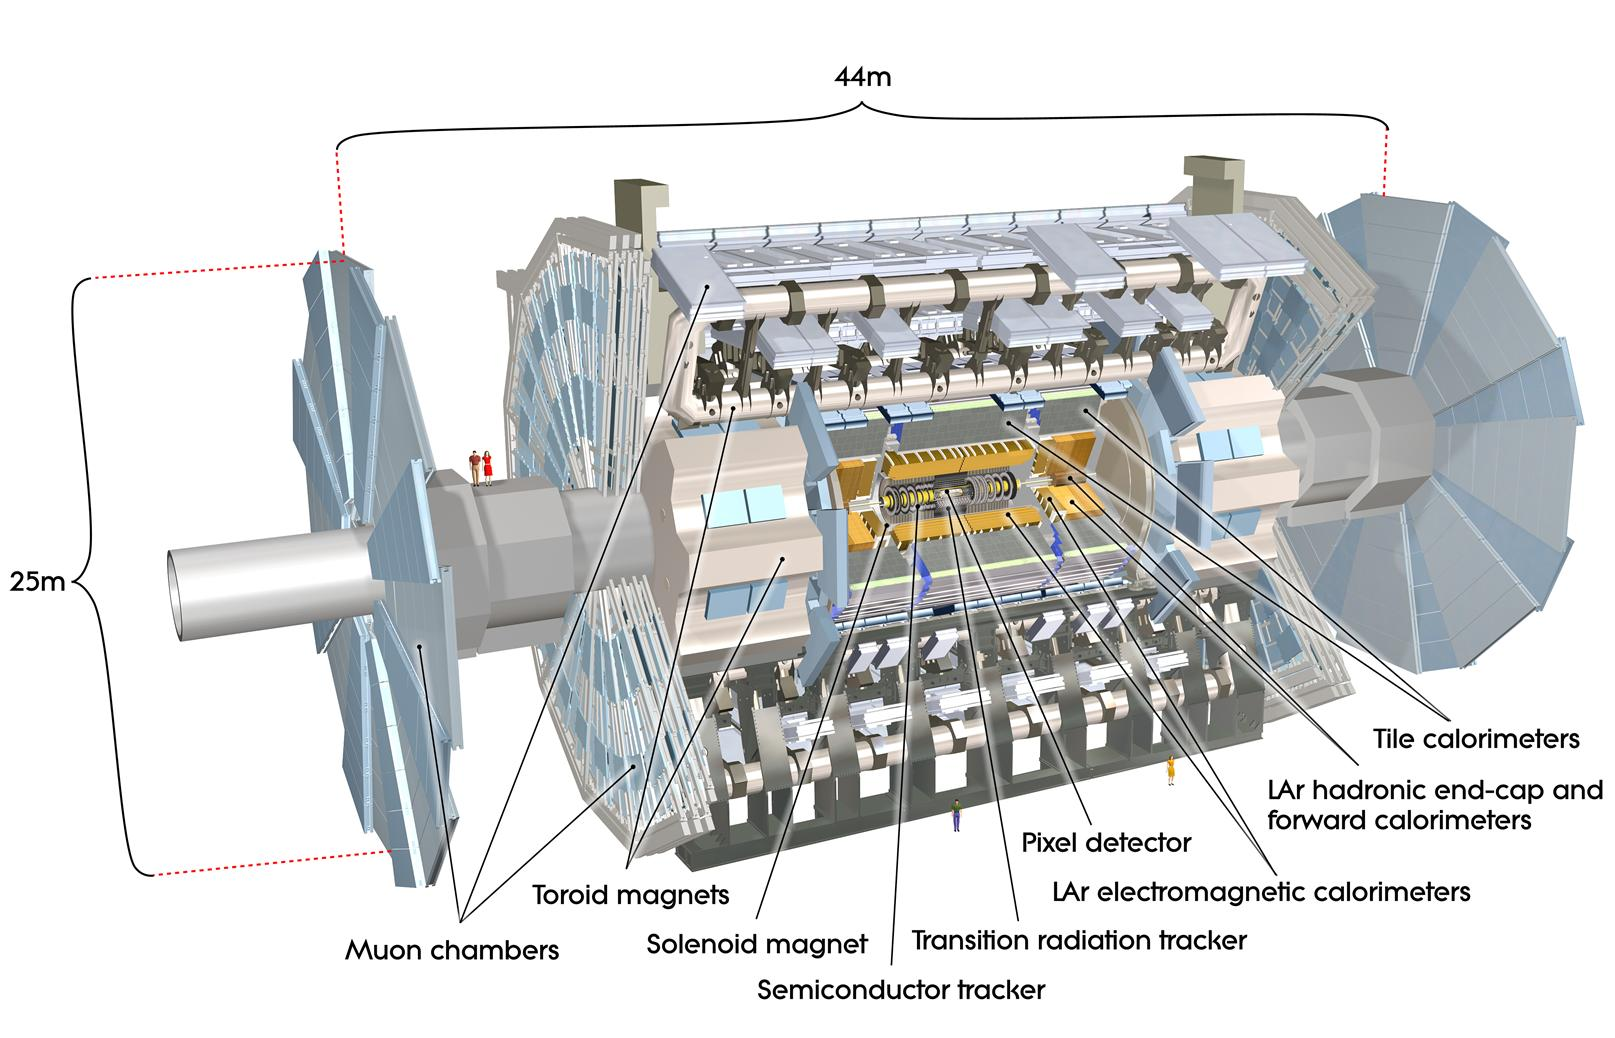
\includegraphics[width=\textwidth]{Chapter2/ATLAS.png}
    \caption{ATLAS detector.}
    \label{fig:ATLASfull}
  \end{subfigure}
  ~
  \begin{subfigure}[b]{0.9\textwidth}
    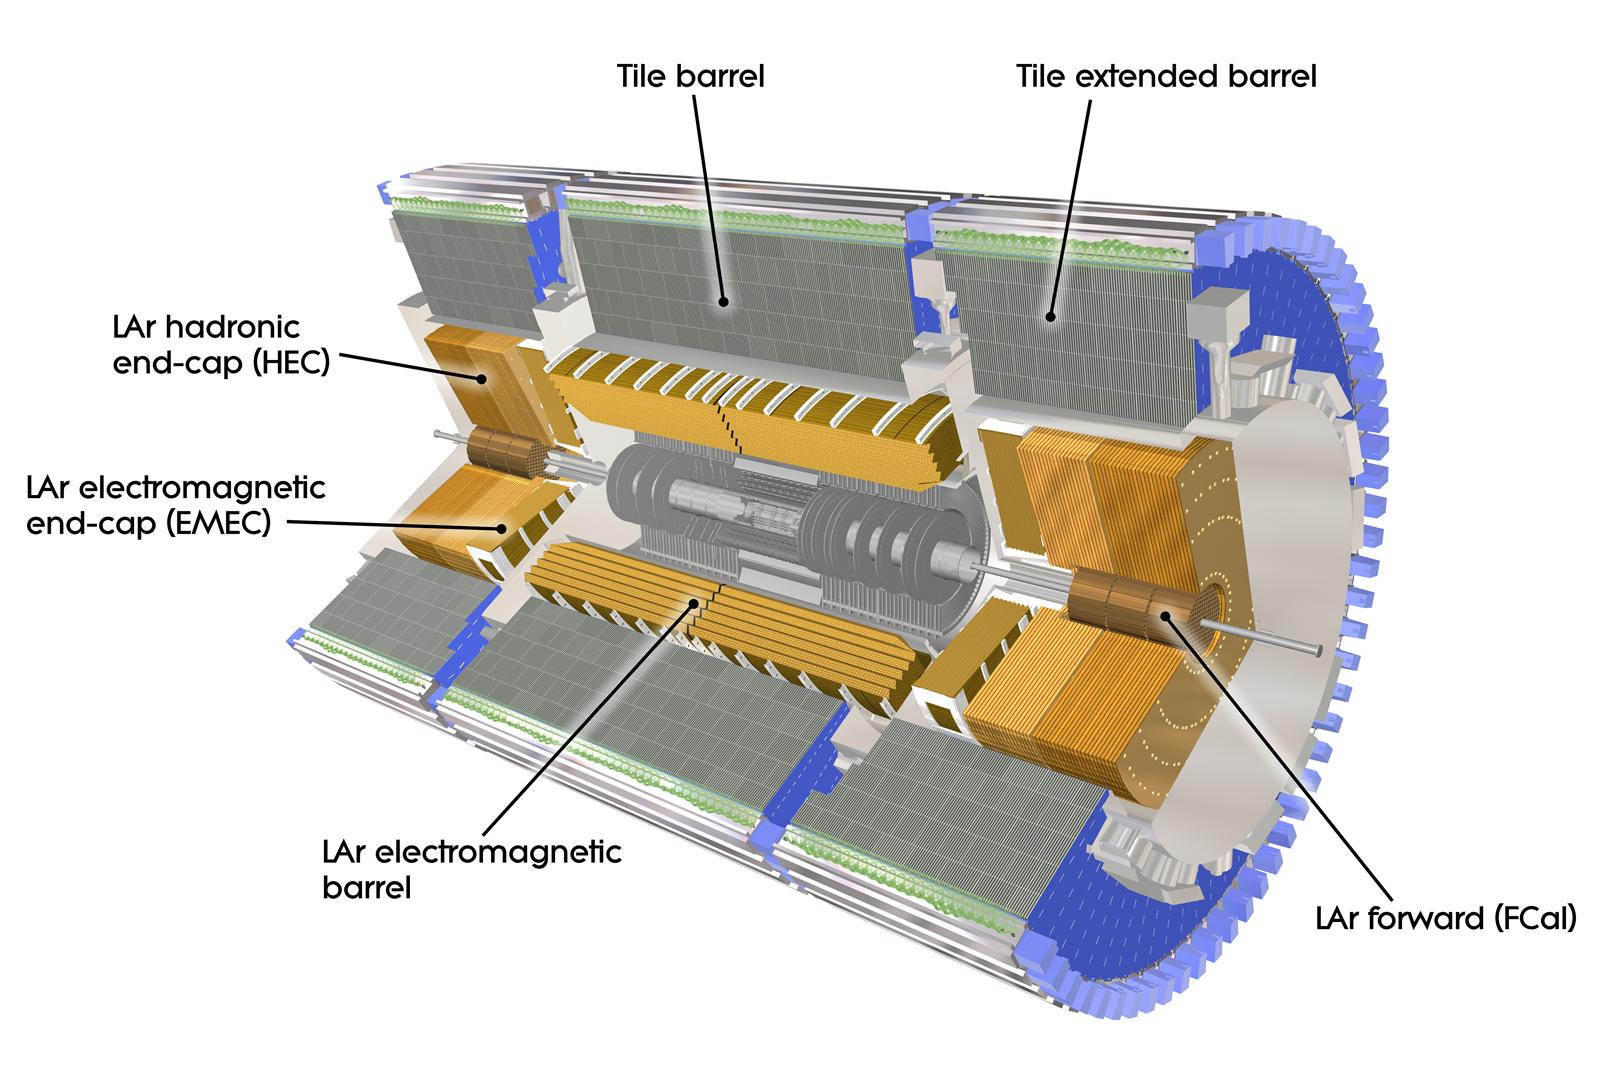
\includegraphics[width=\textwidth]{Chapter2/ATLASinner.jpeg}
    \caption{Inner detector and calorimeter systems.}
    \label{fig:ATLASinner}
  \end{subfigure}
  \caption[(a) An overview of the ATLAS detector 
           (b) Detail on the inner detector and the calorimeters - the dominant
           sub-detector systems used in this thesis.]
           {(a) An overview of the ATLAS detector 
           (b) Detail on the inner detector and the calorimeters - the dominant
           sub-detector systems used in this thesis. Figures taken from
           \cite{CERNbook}.}
  \label{fig:ATLAS}
\end{figure}

ATLAS uses a right-handed coordinate system with its origin at the interaction
point in the center of the detector and the $z$ axis along the beam pipe. The
$x$ axis points from the interaction point to the center of the LHC ring, and
the $y$ axis points upward. Cylindrical coordinates $(r, \phi)$ are used in the
transverse plane, $\phi$ being the azimuthal angle around the beam pipe. Instead
of polar angle $\theta$, pseudorapidity $\eta$ and rapidity $y$ are used in this
thesis.  In the following definitions of pseudorapidity $\eta$ and rapidity $y$,
$E$ stands for the total energy and $p$ for size of total momentum: 

\begin{eqnarray}
  \eta &= & - \frac{1}{2} \ln \left( \frac{p+p_z}{p-p_z} \right) = - \ln \left[
  \tan \left( \frac{\theta}{2} \right) \right], \\ y &= &- \frac{1}{2} \ln
  \left( \frac{E+p_z}{E-p_z} \right).	
\end{eqnarray}
The transverse momentum $\pt = \sqrt{p_x^2 + p_y^2}$ presents the component of a
momentum perpendicular to the beam line.  

The main detector system, relevant to this thesis, is the ATLAS calorimeter system,
which is emphasized in Figure~\ref{fig:ATLASinner}. The calorimeter is divided
into sub-detectors, providing an overall coverage up to $|\eta| < 4.9$. The
electromagnetic calorimeter, covering region $|\eta| < 3.2$, is a
high-granularity sampling detector, in which the liquid argon (LAr) active medium
is interspaced with layers of lead absorber. The hadronic calorimeters are
divided into three sections: a tile scintillator/steel calorimeter is used in
both the barrel ($|\eta| < 1.0$) and extended barrel cylinders ($0.8 < |\eta| <
1.7$), while the hadronic endcap ($1.5 < |\eta| < 3.2$) consists of LAr/copper
calorimeter modules. The forward calorimeter measures both electromagnetic and
hadronic energy in the range $3.2 < |\eta| < 4.9$ using LAr/copper and
LAr/tungsten modules. 

\section{Hadron Collision at the LHC}

Following the Reference about Monte Carlo event generators \cite{PDG} and the
picture in Figure~\ref{fig:HardProcess}, I discuss, in this Section, the
phenomenology of inelastic proton-proton collisions. 

\begin{figure}[t]
  \centering
  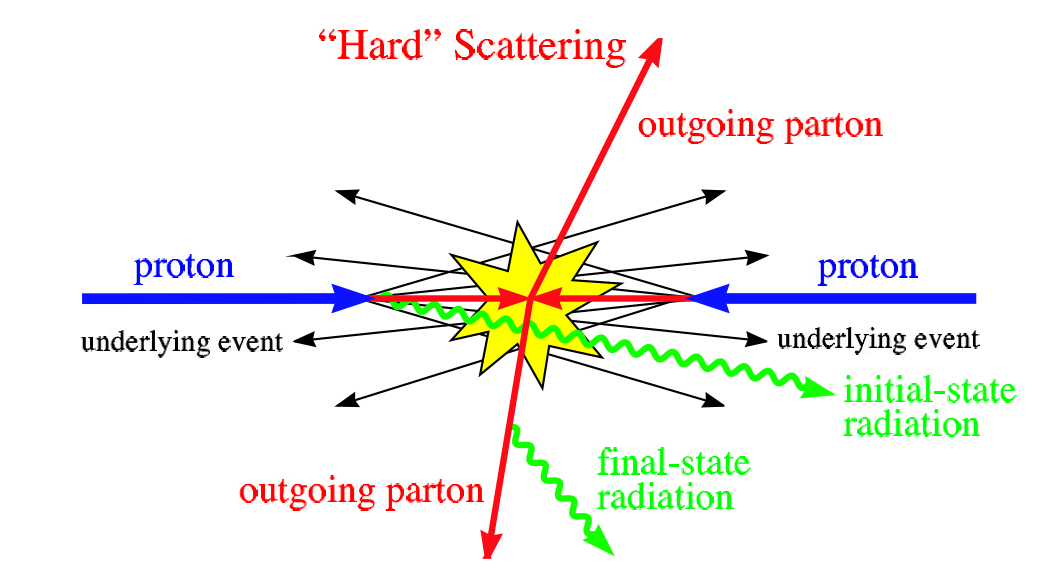
\includegraphics[width=\textwidth]{Chapter2/HardProcess.png}
  \caption[Schematic representation of an inelastic proton-proton
          collision.]
          {Schematic representation of an inelastic proton-proton
          collision. Figure taken from \cite{HardProcess}.}
  \label{fig:HardProcess}
\end{figure}

Two incoming protons can be understood as two bags of partons. 
The inelastic proton-proton collision is dominated by the strong interaction
between two partons, called incoming partons. 
Momentum transfer at their interaction is $Q \gg \Lambda$, co the perturbative
QCD is used to describe the initial process of a hard scattering. 
The remaining energy is carried out by the rest of the partons, which create the so
called underlying event - particles, which do not come from the dominant QCD
processes.

When the partons are sufficiently far from each other, the non-perturbative QCD is
used to describe the process of hadronization, in which a set of colored
partons is transformed into a set of colorless primary hadrons, which may then
decay further. 

During all the collision, the color charges of partons interact, resulting in a
radiation of gluons $q \rightarrow qg$. This process is described by the
perturbative QCD and leads to infrared and collinear divergences. However,
infrared divergences are
canceled by Kinoshita--Lee--Nauenberg theorem \cite{KLN1,KLN2}, so only
collinear divergences remain. There is no mechanism known up to date, which
would solve the problem with collinear divergences. However, observables
inclusive enough, to be insensitive to processes, that distinguish between
different numbers of partons, are not affected by infrared divergences.
There is no possibility, how to theoretically predict the energy of hardest
outgoing particle, but it is possible to predict the energy flow in a cone from
the point of scattering.

This is where the term jet comes to play. A jet can be naively seen as a group
of collimated particles generated by the hadronization of a parton in the
scattering process, and it is the most important object used on hadron colliders for
analysis of QCD processes.

\section{Jet Algorithms}

A jet algorithm is a generic "recipe", which takes a set of particles (or other
objects with defined four-momenta) and returns jets created from them. The jet
algorithm usually involves a set of parameters, which, together with the
algorithm, fully specify the jet definition. According to the remarks at the end
of the previous Section, jet algorithms should fulfill the following conditions 

\begin{enumerate}
  \item Infrared safety - the presence of an additional soft particle should not
    affect the recombination of particles into a jet.
  \item Collinear safety - jet reconstruction should not depend on the fact, if
    the transverse momentum is carried by one particle, or if the particle is split
    into more collinear particles.
\end{enumerate}
Two important steps must be defined in each jet algorithm

\begin{enumerate}
  \item Clustering - description how the input objects are clustered into jets.
  \item Recombination - determination of physical quantities of jets.
\end{enumerate}
Additional steps may include the preclustering, which reduces the number of input
objects for jet algorithm.

This Sections starts with the definition of two classes of jet algorithms.
First of these are cone algorithms, which seems to me to be more
illustrative, and $k_t$ algorithms, which are used in ATLAS experiment. After
a characterization of these algorithms, I introduce two possible recombination
schemes, and, at the end of this Section, I give a short description, how the
objects, defined by its four-momenta, are constructed from the signal
observed on the ATLAS detector. Detailed description as well as other jet
algorithms can be found in \cite{ATLASmain,JetDoporuceniZdenek}.

\subsection{Cone algorithms}

The first step of these algorithms is to order all input objects (reconstructed
detector objects with four-momentum representation) in decreasing order in
transverse momentum $\pt$. If the object with the highest $\pt$ is above a
seed threshold, all objects within a cone in rapidity $y$ and azimuth
$\phi$ with $\Delta R = \sqrt{\Delta y^2 + \Delta \phi^2} < R_{cone}$, where
$R_{cone}$ is the fixed cone radius, are recombined.
A new cone is centered around a new direction and all the objects within the new
cone are recombined and again, the direction is updated. This process continues,
until the direction of the cone does not change anymore after recombination, at
which point, the cone is considered stable and is called a proto-jet. 

At this point, the next seed is taken from the input list and a new proto-jet is
formed with the same iterative procedure. This continues until no more seeds are
available. 

The proto-jets found by this procedure can share some constituents. Constituents
shared between two proto-jets are recombined into a new proto-jet and if the ratio
$E_T^{shared} / \text{min} ( E_T^{neighbor} ) > f$ is over the certain
threshold, for example $f = 0.5$, the neighboring proto-jets are recombined into
one proto-jet (shared constituents are taken only once). If this condition is
not satisfied, the shared constituents are assigned to the nearest proto-jet.
When a proto-jet does not share constituents it is recombined into the jet.

This algorithm is both not infrared safe (Figure \ref{fig:IRsafety}) and not
collinear safe (Figure \ref{fig:ColSafety}). The infrared insensitivity can be
improved by adding the midpoints between pairs of proto-jets fulfilling
$R_{cone} < \Delta R < 2 R_{cone}$ and repeating the iterative procedure with
midpoints being new seeds. Since the collinear unsafety arises from the use of
seed towers, Seedless cone algorithm was developed, which searches the entire
detector to find all stable proto-jets.

\begin{figure}[t]
  \centering
  \begin{subfigure}[b]{0.85\textwidth}
    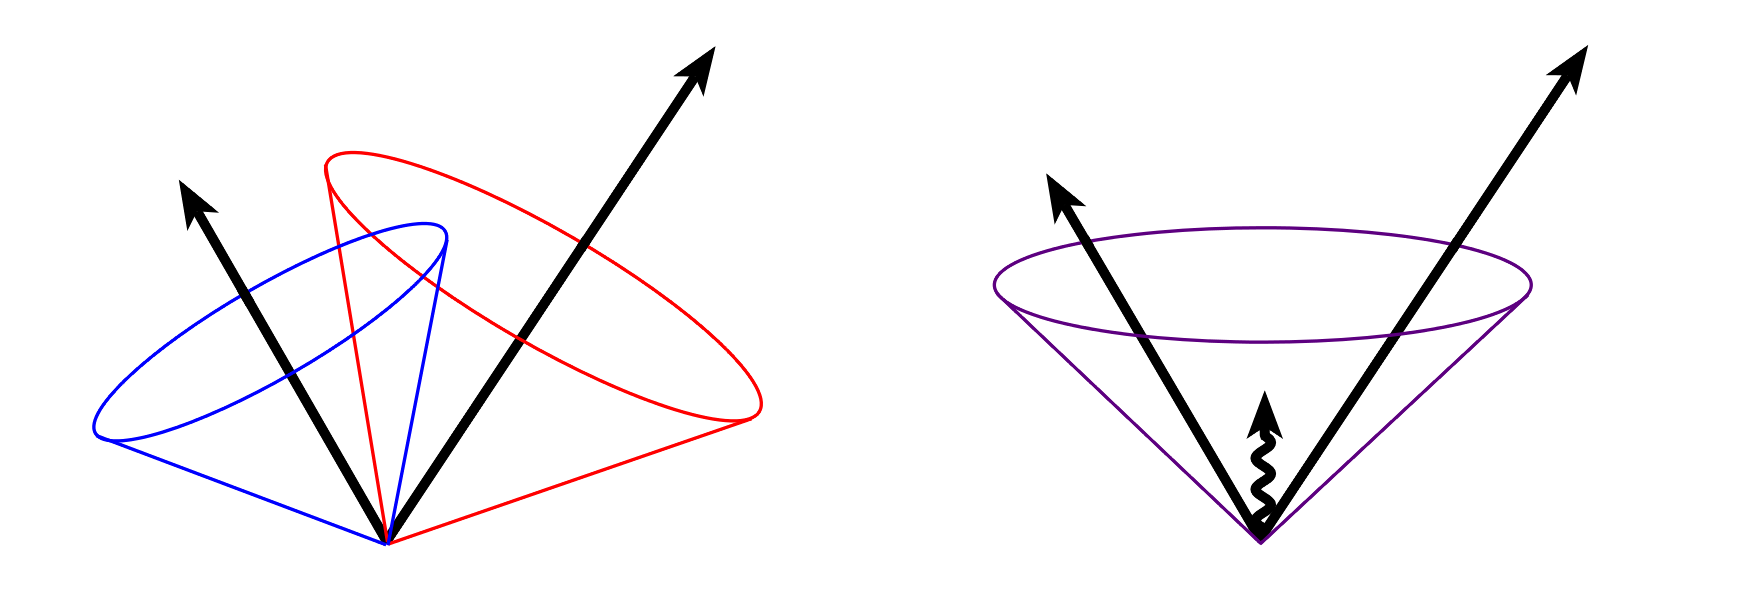
\includegraphics[width=\textwidth]{Chapter2/IRsafety.png}
    \caption{Infrared unsafety.}
    \label{fig:IRsafety}
  \end{subfigure}
  ~
  \begin{subfigure}[b]{0.8\textwidth}
    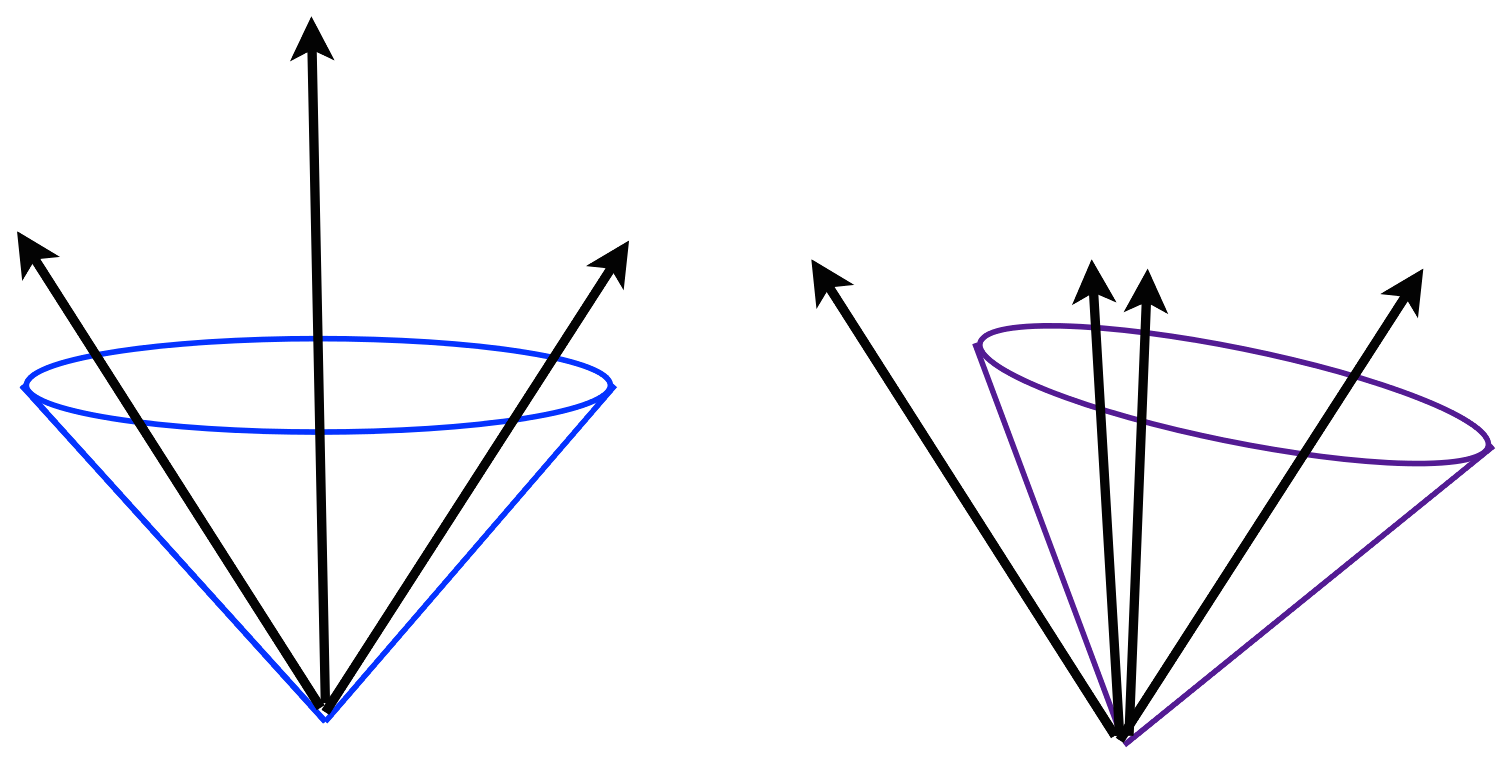
\includegraphics[width=\textwidth]{Chapter2/ColSafety.png}
    \caption{Collinear unsafety.}
    \label{fig:ColSafety}
  \end{subfigure}
  \caption[Illustration of (a) infrared unsafety and (b) collinear unsafety
          of fixed cone jet algorithm.]
          {Illustration of (a) infrared unsafety and (b) collinear unsafety
          of fixed cone jet algorithm.
          Figures taken from \cite{JetTheoreticalPictures}.}
  \label{fig:JetIRCOLsafety}
\end{figure}

Typical parameters used by the fixed cone algorithms are a seed threshold of $\pt > 1 \GeV$,
and a narrow ($R_{cone} = 0.4$) or a wide cone jet ($R_{cone} = 0.7$) option.

\subsection{$k_t$ algorithms}

In this class of algorithms, all pairs $(i,j)$ of input objects are analyzed with
respect to their relative transverse momentum squared, defined by 

\begin{equation}
	d_{ij} = \min{\left( p_{T,i}^{2p} , p_{T,j}^{2p} \right)} \frac{\Delta
    R_{ij}^2}{R^2},
\end{equation}
and the squared $\pt$ of object $i$ relative to the beam axis

\begin{equation}
	d_i = p_{T,i}^{2p}.
\end{equation}
Here $\Delta R_{ij}^2 = (y_i - y_j)^2 + (\phi_i - \phi_j)^2$ and $p_{T,i}$,
$y_i$ and $\phi_i$ are respectively the transverse momentum, rapidity and
azimuth of particle $i$. In addition to the radius parameter $R$, a new
parameter $p$ was introduced, to split $k_t$~algorithms into three categories.  
\begin{itemize}
	\item $p = 1$ $k_t$ algorithm,
	\item $p = 0$ Cambridge/Aachen algorithm,
	\item $p = -1$ anti-$k_t$ jet-clustering algorithm.
\end{itemize}

These algorithms first find the minimum $d_{min}$ of all $d_{ij}$ and $d_i$. If
$d_{min}$ is in $d_{ij}$'s, the corresponding objects $i$ and $j$ are recombined
into a new object $k$ using four-momentum recombination (see
Section~\ref{sse:Recombination}). Both objects $i$ and
$j$ are removed from the list, and the new object $k$ is added to it. If
$d_{min}$ is in $d_i$'s, the object $i$ is considered to be a jet by itself and
is removed from the list.

This means, that all original input objects end up to be either part of a jet, or
to be a jet by themselves. Contrary to the cone algorithms, described earlier, no
objects are shared between jets and the procedure is both infrared and collinear
safe.

ATLAS uses anti-$k_t$ jet algorithm with $R=0.4$ for narrow and $R=0.6$ for wide
jets.  Clustering of calorimeter signal towers (see Section
\ref{sse:CalorimeterJets}) into jets is for $k_t$ and anti-$k_t$ algorithms shown
in Figure~\ref{fig:JetRecombination}.  More information, about differences
between $k_t$~algorithms, can be found, for example, in Reference \cite{ANTIKT}.

\begin{figure}[p]
  \centering
  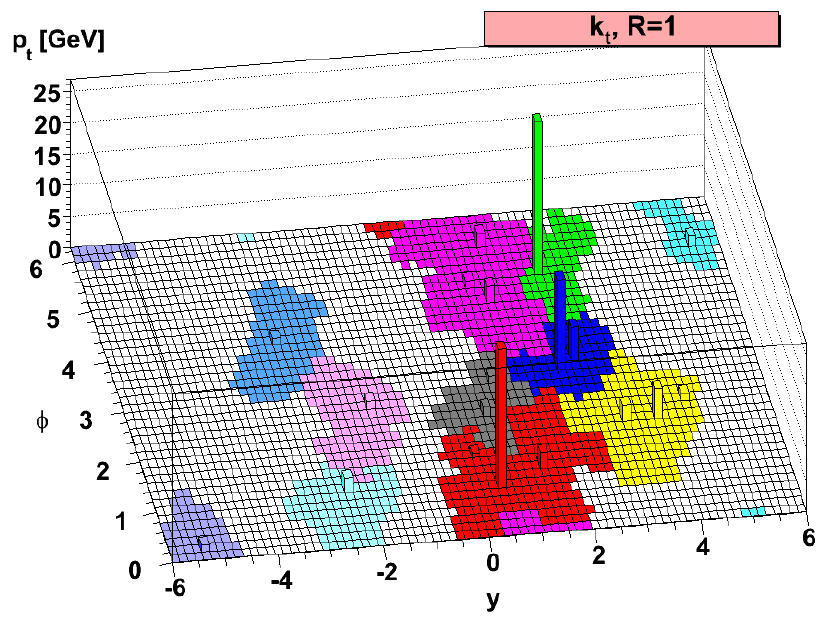
\includegraphics[width=0.9\textwidth]{Chapter2/JetRecombination1.png}
  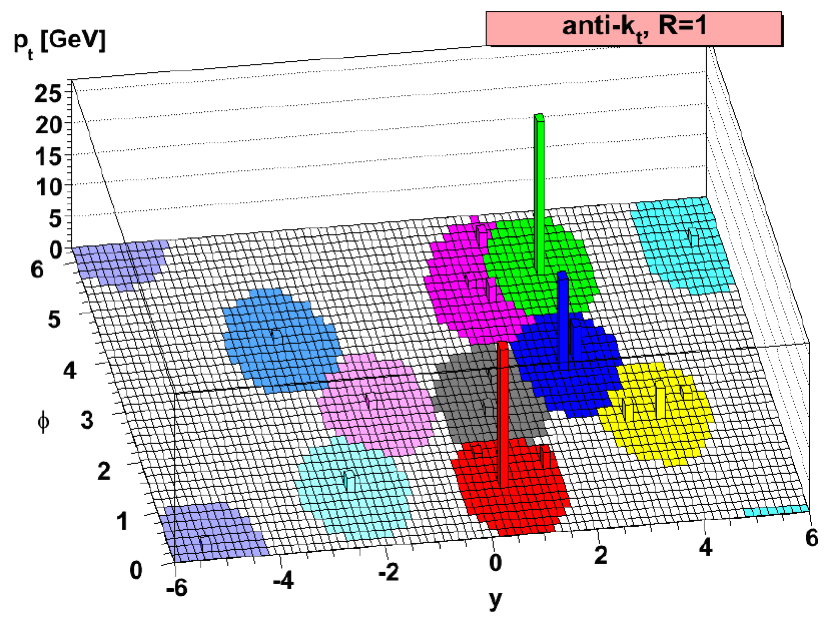
\includegraphics[width=0.9\textwidth]{Chapter2/JetRecombination2.png}
  \caption[Illustration of $k_t$ (top) and anti-$k_t$ (bottom) jet algorithms with $R=1$ for
          calorimeter signal towers in azimuthal angle $\phi$ and pseudorapidity $y$. Towers of
          the same color were clustered into one jet. ]
          {Illustration of $k_t$ (top) and anti-$k_t$ (bottom) jet algorithms with $R=1$ for
          calorimeter signal towers in azimuthal angle $\phi$ and pseudorapidity $y$. Towers of
          the same color were clustered into one jet. Figures taken from
          \cite{JetTheoreticalPictures}.} 
  \label{fig:JetRecombination}
\end{figure}

\subsection{Recombination}
\label{sse:Recombination}

Let $J$ be the index set of the input objects with the defined four-momenta
$(E^i,p_x^i,p_y^i,p_z^i)$, $i \in J$ which has to be recombined into the jet
with new kinematic quantities $E^J$, $\mathbf{p}^J$, $\pt^J$, $y^J$, $\ldots$
Possible recombination schemes are

\begin{itemize}
\item \textbf{Snowmass Scheme}

Used by fixed cone algorithm when finding proto-jets.

\begin{equation}
  E_T^J = \sum_{i \in J} E_T^i
  \quad , \quad
  \eta^J = \frac{1}{E_T^J} \sum_{i \in J} E_T^i \eta^i
  \quad , \quad
  \phi^J = \frac{1}{E_T^J} \sum_{i \in J} E_T^i \phi^i.
\end{equation}

\item \textbf{Four-Momentum Recombination ($E$-Scheme)}

Used by $k_t$-algorithms and by fixed cone algorithm to final recombination of
proto-jets into jets.

\begin{equation}
  p^J = ( E^J, \mathbf{p}^J ) = \sum_{i \in J} (E^i,p_x^i,p_y^i,p_z^i),
\end{equation}
\begin{equation}
  \pt^J = \sqrt{(p_x^J)^2 + (p_y^J)^2}
  \quad , \quad
  y^J = \frac{1}{2} \ln \frac{E^J + p_z^J}{E^J - p_z^J}
  \quad , \quad
  \phi^J = \tan^{-1} \frac{p_y^J}{p_x^J}.
\end{equation}
\end{itemize}

\subsection{Calorimeter jets}
\label{sse:CalorimeterJets}

The ATLAS calorimeter system, with $\sim 200,000$ individual cells, is the most
important detector system for the jet reconstruction. Calorimeter cells differ
in sizes, geometries, as well as in readout technologies, and for jet algorithms,
these cells has to be firstly combined into larger objects, having physically
meaningful four-momenta. The two concepts available are the calorimeter signal
towers and the topological cell clusters, which I will describe shortly.

In the case of calorimeter signal towers, the cells are projected onto a fixed
grid in pseudorapidity $\eta$ and azimuth $\phi$. The tower bin size is $\Delta
\eta \times \Delta \phi = 0.1 \times 0.1$ in the whole acceptance region of the
calorimeters, i.e. in $|\eta| < 5$ and $- \pi < \phi < \pi$ with approximately 
$100 \times 64 = 6400$ towers in total.

The second possibility, how to combine calorimeter cells into a larger objects,
are the topological cell clusters, which are an attempt to reconstruct a
three-dimensional "energy blobs" created by each of the particles entering the
calorimeter.  The clustering starts with a seed cells with a signal-to-noise
ratio, or signal significance $\Gamma = E_{cell} / \sigma_{noise,cell}$, above a
certain threshold $S$, for example $|\Gamma| > S = 4$.  All directly neighboring cells
of these seed cells, in all three dimensions, are collected into the cluster.
Neighbors of neighbors are considered for those added cells which have $\Gamma$
above a certain secondary threshold $N$, for example $|\Gamma| > N = 2$. Finally, a ring of
guard cells with signal significances above a basic threshold $|\Gamma| > P$ is
added to the cluster. After the initial clusters are formed, they are analyzed
for local signal maxima by a splitting algorithm, and split between those
maxima.

\section{Jet corrections}

Before jets can proceed to the data analysis, corrections have to be applied to
minimize detector effects including calorimeter non-compensation, noise, losses
in dead material and cracks, longitudinal leakage and particle deflection in the
magnetic field. Indispensable tool for jet corrections are Monte Carlo event
generators - \textsc{Pythia8} \cite{Pythia8} generating high-energy-physics
events and \textsc{Geant4} \cite{Geant4} or \textsc{AtlfastII} \cite{AtlfastII}
detector simulations for simulating the ALTAS detector response of
\textsc{Pythia8} generated events.

Using these tools, it is possible to reconstruct jets from Monte Carlo events on three
different stages of collision indicated in Figure~\ref{fig:JetPhases}. Firstly,
there are parton jets, which are reconstructed from the quarks, gluons and other
elementary particles created just after the collision. Stable particles (with
lifetime $c\tau \sim 10^{-15}\,\text{m}$), created by hadronization, are recombined into
the truth jets. When a collision reaches the detector, the detector simulation
is used and the recorded signal is reconstructed into reco jets.
The objective of the jet corrections is to find universal prescription, how to
modify a reco jet properties, to observables derived from detector level,
correspond to the observables on particle level.

\begin{figure}[t]
  \centering
  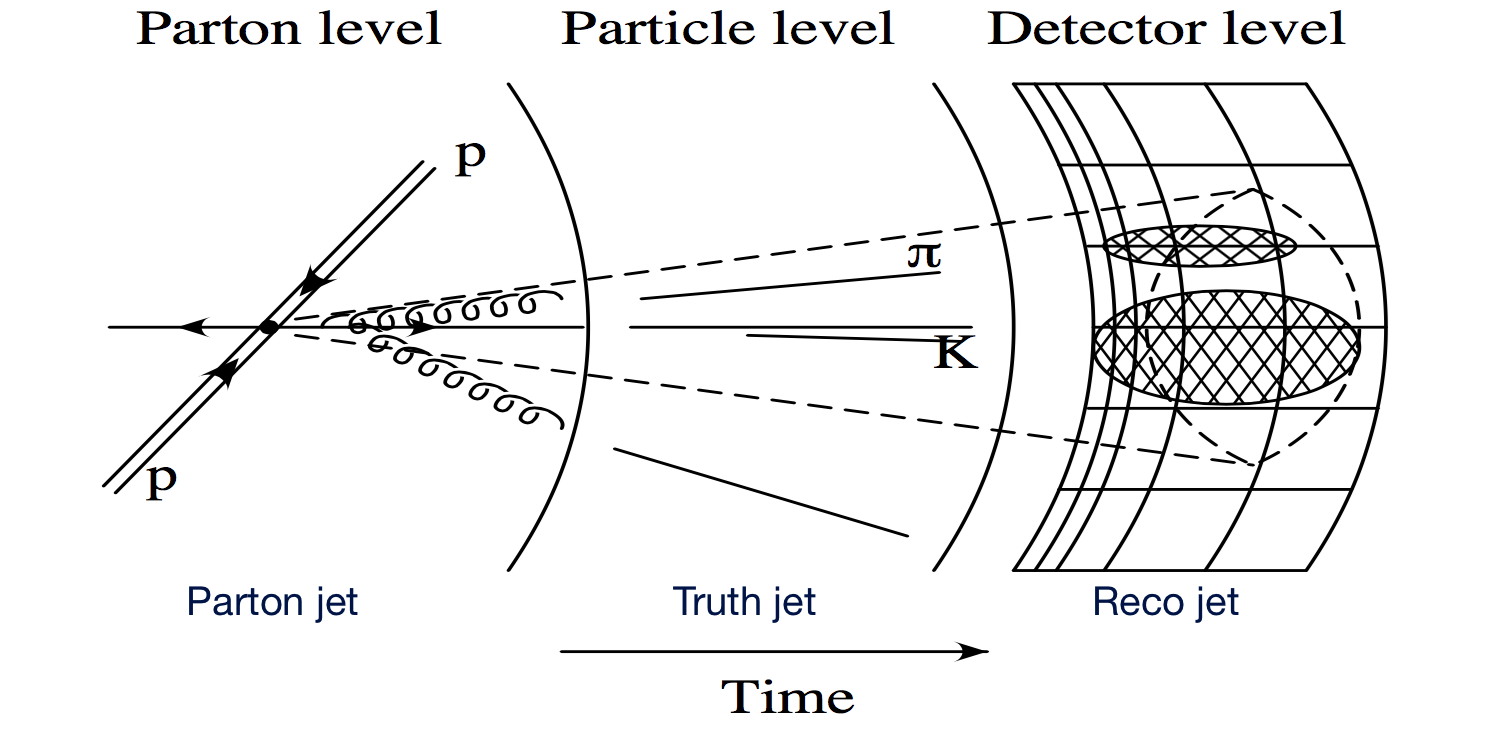
\includegraphics[width=\textwidth]{Chapter2/JetPhases.png}
  \caption[Three levels of jet reconstruction.]
    {Three levels of jet reconstruction. Figure taken from \cite{ZdenekThesis} } 
  \label{fig:JetPhases}
\end{figure}

Firstly, the reco jets are corrected to the truth jets leading to a modification
of kinematic properties of the individual reco jet in the process called jet energy
scale calibration.
There are, however, some detector effects, which can not be
fixed by this calibration. These effects include the limited detector resolution
(detector cells have finite dimensions) and the limited acceptance (not all
events are recorded). The former leads to the smearing of jet kinematic
properties, whereas the later to decrease of observed cross section against the
cross section theoretically expected. Both of these effects are negatively affecting the
observables and can be partially removed by the unfolding procedure, which,
unlike the jet calibration, is analysis dependent.

\subsection{Jet Energy Scale Calibration}

Energy $E_{reco}$ of the jet measured by the detector may differ from the energy
$E_{truth}$ of the corresponding particle jet. The goal of the jet energy scale
calibration is to remove some detector effects and correct $E_{reco}$ to
$E_{truth}$. The detector effects can be summarized by the formula

\begin{equation}
  E_{truth} = \frac{E_{reco} - O}{R \cdot S},
\end{equation}
where the following corrections was defined

\begin{itemize}
  \item \textbf{Offset} $\mathbf{O}$
  \\*
    Represents the subtraction of additional energy, which is represented by the
    detector noise and pile-up with contributions from other proton-proton
    collisions, occurring during beam crossing.

  \item \textbf{Response} $\mathbf{R}$
  \\*
    Describing a fraction of a truth energy, which was measured by the
    detector. Thanks to the hadronic character of jets observed at the LHC, this
    is the largest correction.

  \item \textbf{Showering} $\mathbf{S}$
  \\*
    Characterizing particle flow out/from jet recombination cells.

\end{itemize}

More concise information about the parameters, just introduced, can be found in
\cite{ZdenekThesis}.

Because the calibration is persistently evolving, each jet analysis uses as an
input the uncalibrated reco jets, which are then easily calibrated using
standard \textsc{ApplyJetCalibration} library \cite{ApplyJetCalibration}.

\subsection{Theory of Unfolding}

In this analysis, the distribution $f(\pt)$ of inclusive jet $\pt$ is measured
for $\pt \in \langle a, b \rangle$. Due to the detector imperfections,
instead of physical variable $\pt$, a new variable $x$ and its distribution
$g(x)$ are measured. The measured distribution can be expressed as

\begin{equation}
  g(x) = \int_a^b A(x, \pt) f(\pt) d\pt,
  \label{eq:UnfoldingBasicDefinition}
\end{equation}
with the function $A(x, \pt)$ describing the detector response, as it can be
seen, when the detector is exposed to a particle beam with well known $\pt =
\pt'$, meaning $f(\pt) = \delta(\pt - \pt')$, leading to $g(x) = A(x, \pt')$. The
reconstruction of $f(\pt)$ from measured $g(x)$ is called unfolding.

For practical purposes, the equation \eqref{eq:UnfoldingBasicDefinition} should
be discretized, so, instead of continuous distribution $g(x)$, the discretized
values $g_i = \int_{N(i)} g(x)dx$ of discretized observable $f_i =
\int_{N(i)} f(\pt)d\pt$ are measured. Here, the integration is done over
measurable $N(i) \subset \langle a, b \rangle$. For simplicity, assume $x \in
\langle a, b \rangle$ is discretized in the same way as the physical $\pt$.
Equation \eqref{eq:UnfoldingBasicDefinition} then reads

\begin{equation}
  g = Af,
  \label{eq:UnfoldingDiscretized}
\end{equation}
with $g$ and $f$ being vectors of $g_i$'s and $f_i$'s respectively and $A$
matrix derived from $A(x, \pt)$. This matrix is later, in Section
\ref{Sec:Unfolding3}, called the transfer matrix. If the limited acceptance
would be the only detector problem, then $A$ would be a diagonal matrix with some
elements $ < 1$. When the limited resolution comes to play, the diagonal entries
start to smear out of the diagonal and the matrix $A$ starts to complicate.

The unfolding results which offers the solution of
\eqref{eq:UnfoldingDiscretized} by the inversion of matrix $A$, are mostly
disappointing, as is illustrated e.g. in \cite{UnfoldingExplained}. To improve
results, different unfolding methods were developed. These include Iterative
Bayesian Unfolding \cite{IterativeBayesianUnfolding}, Singular Value
Decomposition \cite{SingularValueDecomposition}, or Iterative, Dynamically
Stabilized (IDS) method \cite{IterativeDynamicallyStabilized}, which is the
method, I have used in this thesis. 


